%%This is a very basic article template.
%%There is just one section and two subsections.
\documentclass{thesis}

\usepackage{makeidx}
\usepackage[T1]{fontenc} 
\usepackage[ngerman]{babel}
\usepackage[utf8]{inputenc}
\nonfrenchspacing
\usepackage{url}
\usepackage{breakcites}
\usepackage{epsfig} 

\begin{document}
\pagenumbering{roman}
\title{Generierung einer frontendseitigen GWT Anwendung unter Verwendung
von dem MVP Pattern und Dependency Injection}
\author{Claudia Schäfer	|	Marcus Fabarius	|	Stephanie Lehmann\\ CMS}
\maketitle


 % The page style headers have been "empty" all this time, now use the "fancy" headers as defined before to bring them back

 % Set the left side page header to "Contents"
\tableofcontents % Write out the Table of Contents

\pagenumbering{arabic}
\chapter{Einleitung}
\label{Einleitung}
Dieses Projekt entstand im Rahmen des Software Engineering - Advanced Topic
Kurses im Master Studiengang Medieninformatik, der Beuth Hochschule Berlin, im
Wintersemester 2013/14.

Die Ausarbeitung beschäftigt sich mit der Generierung eines Google Web
Toolkit (GWT) Projektes.
Dies erfolgt durch eine Model-To-Text Transformation mittels eines Model
Transformation Language (MTL) Generators, welchem mit der Object Constraint Language (OCL), weitere
Funktionalitäten zur Verfügung stehen. 

Dabei wird ein besonderes Augenmerk auf die Architektur gelegt, allerdeings ohne
des Einsatzes von Layouting. Deshalb findet eine Generierung anhand einer
vorgegebenen Grundstruktur bzw. -architektur statt. Mit dem in der vorliegenden
Projektarbeit entwickelten Generator, ist es einem Entwickler möglich eine
komplette GWT Struktur generieren zu lassen. Auf Grundlage eines, auf einem UML
Profil basierenden, Klassendiagramms kann eine komplette GWT Frontend
Webanwendung abgebildet und mit kleinen Änderungen schnell lauffähig gemacht werden.
Das UML Profil wird so gestaltet, dass eine GWT Anwendung gemäß der vorgegebenen
Architektur einfach umgesetzt werden kann. Dabei finden das
Model-View-Presenter (MVP) Pattern sowie verschiedene Frameworks, welche
weiterhin Architekturkonzepte, beispielsweise für Dependency Injection, liefern,
als grundlegende Konstrukte Verwendung. Anstoß zu diesem Projekt war eine
gegebene \glqq{}Best Practice\grqq{} Lösung mehrerer Entwickler, die jedoch
ziemlich aufwändig und fehleranfällig in der Umsetzung ist.
\\\\
In dem weiterem Verlauf dieser Ausarbeitung werden die zugrundeliegenden
Konzepte und Frameworks (vgl. Abschnitt \ref{Grundlagen}) vorgestellt. Weiterhin
wird die Idee und konzeptionellen Aspekte (vgl. Abschnitt \ref{Konzeption}),
auch hinsichtlich der Ziel-Architektur, erläutert. Diese werden im
Weiterem mit sich ergebenden Änderungen umgesetzt (vgl. Abschnitte \ref{UMLProfil},
\ref{M1Modell}, \ref{Generator}).
Anhand des Ergebnisses (vgl. Abschnitt \ref{Ergebnis}) wird gezeigt, dass eine
GWT Anwendung anhand zweier Anwendungsfälle generiert und wie diese lauffähig
gemacht werden kann. Zusammenfassend folgt eine Bewertung des Generator
Projektes mit einem Ausblick auf Erweiterungsmöglichkeiten (vgl. Abschnitt
\ref{FazitAusblick}).

\chapter{Grundlagen}
\label{Grundlagen}

Text\ldots
% ---------------------------------------------
% MDA
% ---------------------------------------------
\section{Model Driven Architecture} \label{MDA}
Model Driven Architecture (dt. Modellgetriebene Architektur), kurz MDA, stellt
einen Ansatz zur Softwareentwicklung dar. Dieses Konzept ist 2001 von der
Object Management Group (OMG) veröffentlicht worden und gilt heute als
Standard. Hierbei werden Richtlinien zur Spezifikation in Form von Modellen vorgegeben.
Aus diesen Modellen, die formal eindeutig sind, wird dann mithilfe von Generatoren
automatisch der benötigte Code erzeugt. Ziel der MDA-Architektur ist es, den gesamten Prozess der Softwareerstellung in möglichst plattformunabhängigen Modellen darzustellen, sodass die Software zu einem hohen Anteil automatisch durch Transformationen von Modellen erzeugt werden kann. Die dabei entstehenden Transformatoren können eine hohe Wiederverwendbarkeit und Wartbarkeit sicherstellen.\cite[S. 79 f.]{bib:MDA1}\\
Bei den Modellen handelt es sich im Speziellen, um das Platform Independent Model und das Platform Specific Model, welche bei diesem Projekt auf das Metamodell der UML 2.4 Anwendung fanden.
Was dies genau bedeutet und wie die verschiedenen Modelle zu verstehen sind, wird in dem folgenden Abschnitt erläutert

\subsection{Platform Independent Model}
\label{PIM}
\subsection{Platform Specific Model} \label{PSM}
Kombiniert man die Funktionalitäten, die im Platform Independent Model definiert
sind, mit den Designanforderungen der gewünschten Plattform, so erhält man das
Platform Specific Model (PSM, dt. Plattformspezifisches Model). Im Gegensatz zum
PIM, welches nur die fachlichen Anforderungen definiert, werden beim PSM auch
die technischen Aspekte eingebunden.
% ---------------------------------------------
% GWT
% ---------------------------------------------
\section{GWT}
\label{GWT}
Das Google Web Toolkit, kurz GWT, ist ein open-source Projekt von Google. Es
dient der Entwicklung von Webanwendungen mittels Java. Dabei übersetzt der GWT
Compiler den gesamten Java Source-Code in JavaScript Code.
Zudem werden während der Übersetzung Code Optimierungen vorgenommen, welche u.A.
das Löschen von nicht benötigtem Code, z.B beim Einsatz von mehreren
Browsern als Plattformen, betreffen. 

Weiterhin bietet GWT die Möglichkeit zur Interaktion mit JavaScript durch
das JavaScript Native Interface, kurz JSNI.
Dadurch können JavaScript Bibliotheken angebunden bzw. verwendet oder die
Nutzung von JSON erleichtert werden \cite[S. 4-9]{bib:GWTinAction}\cite[S.
237-238]{bib:GWToReilly}.

Darüber hinaus ist dadurch eine Kommunikation mit dem Backend
möglich. Zusätzlich kann diese Kommunikation durch Remote Procedure Calls,
kurz RCPs, u.A. mittels RequestBuilder oder GWT-RCP erfolgen. Beide setzen auf
dem XMLHttpRequest JavaScript Objekt auf, welches die Kommunikation zwischen dem
Browser und dem Server ohne Seitenneuladen erlaubt. Der RequestBuilder ist ein
Wrapper für das genannte JavaScript Objekt und GWT-RCP ermöglicht den Austausch
von konkreten Java Objekten \cite[S. 16]{bib:GWTinAction}\cite[S.
222]{bib:GWToReilly}.

Dies zeigt einen kurzen Einblick in die verschieden Möglichkeiten mit
GWT, welche folgend nicht näher erläutert werden, weil eine Generierung einer
GWT Frontend Anwendung ohne Server Kommunikation erfolgen soll.

Der Einsatz mit GWT ist flexibel und durch den GWT Compiler wird 
eine bessere Laufzeitausfürhung der Webanwendung erlangt\cite{bib:GWTStarted}.
Dies sind 2 Vorteile des Nutzens von GWT. Zusätzlich sind die durch Google
gebotenen Architekturkonzepte durch u.A. Model-View-Presenter, kurz MVP, ein
Ansatz und Grund einen Generator für GWT Frontend Anwnedungen zu schreiben.
Dafür werden im weiterem Verlauf MVP, UiBinder sowie GIN erläutert, welche die
Grundlage der umzusetzenden Architektur bilden.

\subsection{MVP}
\label{MVP}
MVP (Model-View-Presenter) ist ein Design Pattern. Es ist ähnlich dem MVC
(Model-View-Controller). Google beschreibt den Nutzen des MVP Patterns in der
Einbindung von Testfällen in einer GWT Anwendung. Darüber hinaus kann dieses
Pattern auch genutzt werden um eine GWT Anwendung für verschiedene Plattformen
verfügbar zu machen z.B. für Browser auf mobilen Endgeräten oder auf dem
Desktop.
\begin{figure}[htbp]
\begin{center}
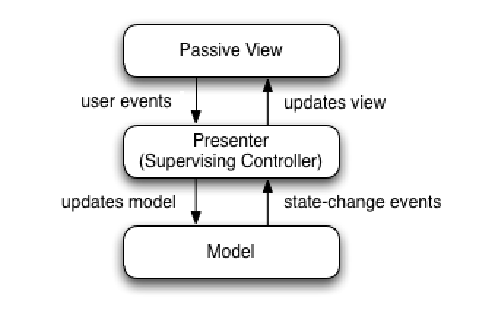
\includegraphics{./img/MVP.pdf}
\caption{Visualisierung des MVP Patterns \cite{bib:MVP1}}\label{Fig:MVP}
\end{center}
\end{figure}\\
Bei MVP übernimmt der Presenter die Logik und die View ist einfach gehalten
\cite{bib:MVP2}. Dies sorgt für eine klare Trennung zwischen Model und View (vgl.
Abbildung \ref{Fig:MVP}). Wohingegen bei MVC die View das Model kennt
\cite{bib:MVCvsMVP}. Der Presenter steuert die View und übermittelt die Daten
des Models zur View.
Dadurch wird der einfache Austausch von Views ermöglicht ohne das weitere
Änderungen vorgenommen werden müssen \cite{bib:MVP1}\cite{bib:MVP2}.

In der zu generierenden Anwendung soll das MVP Pattern ohne ein konkretes Model
implementiert werden, da ausschließlich eine GWT Frontend Anwendung generiert
werden soll. Die MVP Struktur ist dabei so umgesetzt, sodass der Presenter als
Interface in dem View Interface enthalten ist und über eine Activity definiert
wird, welche zusätzlich für das Event handling und die Datenbeschaffung verantwortlich
ist. Die konkrete Implementierung der View beinhaltet das Presenterobjekt, damit
dadurch die Aktionen der View Komponenten (bei GWT Widgets) an den Presenter
übergeben werden können.

\subsection{UI-Binder}
\label{UIBinder}
% ---------------------------------------------
% GIN
% ---------------------------------------------
\section{Dependency Injection mittels GIN} \label{GIN}
Bei Dependency Injection handelt es sich um einen Begriff aus der
objektorientierten Programmierung, welcher zuerst von Martin Fowler 2004
verwendet worden ist \cite{bib:DI}. Beim Dependency Injection handelt es sich um
ein Verfahren, bei dem zur Laufzeit eines Programmes zusätzliche Informationen,
beispielzweise beim Aufruf einer Funktion, zur Verfügung gestellt werden. Dies
wird von einem extra Dependency Injection Framework vorgenommen, in dieser
Arbeit wird handelt es sich dabei um das GIN Framework.

\subsection{GIN}
Das GIN-Framwork, ist ein Framwork für Dependency Injection, es wurde von Google
für GWT entwickelt \cite[GIN]{bib:gin}. GIN setzt auf Google Guice
\cite[Guice]{bib:guice} auf und erweitert die Java Dependency Injection für den
speziellen Anwendungsfall von GWT.  GIN wurde direkt in den GWT Generator
eingebaut, wodurch es möglich ist die Dependency Injection teilweise schon zur
Compile Zeit einzufügen, dies Sorgt dafür das es kaum Laufzeit Overhead gibt.

Guice wurde 2008 von Google für Dependency Injection mit Java entwickelt und war
das erste Framwork, das Dependency Injection mit Hilfe von Annotationen
ermöglicht hat. Bei Guice werden mittels bind-Befehlen eine Verbindung zwischen
Interfasen und deren konkreten Klassen hergestellt, dadurch sind die konkreten
Implementierungen leichter Austauschbar.


\chapter{Idee}
\label{Idee}
In erster Linie soll eine GWT Frontend Anwendung generiert werden, basierend auf
einer vorgegebenen Architektur (vgl. Abschnitt \ref{AufBZielArchitektur}). Dabei
ist eines der Hauptziele die leichte Erstellung der GWT Anwendung, ohne
Abhängigkeiten zu der zu generierenden Architektur. Darüber hinaus sollen
Vorteile durch vorgegebene Architekturpatterns wie der leichte Austausch von
Ansichten durch MVP weiterhin nutzbar sein. Zusätzlich ist es wünschenswert, das
Verhalten von View Komponenten wie Buttons z.B. für eine Navigation innerhalb
der Ansichten zu ermöglichen. Weitere dieser Verhaltensspezifikationen können
das öffnen eines Popup's sowie die Übertragung von Daten sein. Auch hierbei
steht die einfache Erstellung einer GWT Anwendung und die Konformität
der Architektur im Vordergrund.

Es sollen alle von GWT vorgegebenen View Komponenten wie Buttons, Label und
Menubars für den Entwickler verwendbar sein, welche zusätzlich
untereinander zugeordnet werden können. Des Weiteren sollen Elemente, die auf
jeder Ansicht zu sehen sind, wie z.B. ein Header implementiert werden. Dabei
werden Layout- und Stylevorgaben nicht berücksichtigt, da dafür UI-Editoren
existieren, mit denen eine \grqq{}schöne, gestylte\grqq{} Ansicht ermöglicht wird.

Es sollen weitere eigene View Komponenten erstellt werden können, damit,
unabhängig der vorgegebenen Architektur, weitere architektonische Maßnahmen
erfolgen können. Dazu zählt zum Beispiel die Erstellung einer Datentabelle,
welche mehrmaligen Einsatz innerhalb der Anwendung findet. Darüber hinaus soll
eine vorgegebene Paketierung sowie selbsterstellte Paketetierung für Views
generiert werden.

Zur Erstellung einer GWT Frontend Anwendung soll ein UML-Modell
erstellt werden (vgl. Abschnitt \ref{AufBM1}), basierend auf dem zum
Generator-Projekt gehörendem UML-Profil (vgl. Abschnitt \ref{AufBProfil}),
welches durch den Generator (vgl. Abschnitt \ref{AufBGenerator}) generiert
werden soll.
% ---------------------------------------------
% Konzepte
% ---------------------------------------------
% ---------------------------------------------
% ZielArchitektur
% ---------------------------------------------
\section{Ziel-Architektur}\label{AufBZielArchitektur}
Die für die Generierung vorgesehene Architektur basiert auf 
Architekturkonzepten verschiedener Entwickler und entstand bei der Entwicklung
von vorhergehenden GWT Projekten. Diese Architektur stellte sich dabei als Best
Practice Lösung heraus, welche jedoch aufwändig und fehleranfällig bei der
Umsetzung ist. Dies ist einer der Gründe einen Generator für GWT Frontend
Anwendungen zu entwickeln. Im Folgendem wird die umzusetzende Architektur
kategorisiert und anhand der zu erstellenden Klassen und Dateien vorgestellt.
% -------------------Struktur Erklärungen--------------------------
\begin{itemize}
  \item einmalig vorhandene Dateien und Klassen
  \begin{itemize}
    \item \textbf{index.html}\\
    HTML Seite über die, durch GWT, die in Java erzeugten View Klassen
    eingebunden werden.
    \item \textbf{styles.css}\\
    CSS Datei für die Festlegung der Style-Eigenschaften.
    \item \textbf{\grqq{}Name\grqq{}.gwt.xml}\\
    Konfigurationsdatei in der u.A. verwendete Bibliotheken sowie
    Browsereinstellungen und die Zugriffsklasse eingetragen wird.
    \item \textbf{AppEntryPoint.java}\\
    Zugriffsklasse, d.h. die Einstiegsklasse für die GWT Anwendung. In dieser
    Klasse wird u.A. die ContentView sowie die PermanentViews und die
    HistoryMapper definiert.
    \item \textbf{AbstractView.java}\\
    Ist die Oberklasse aller View Klassen Implementierungen innerhalb der
    esrtellten GWT Anwendung. Diese definiert Eigenschaften für alle Views und
    ermöglicht als Oberklasse den Austausch der
    Ansichten.-----------------------------------
    \item \textbf{AbstractActivityDefaultImpl.java}\\
    Diese Klasse wird von allen View Activity Klassen erweitert und dient
    mittels \textit{start}-Methode dazu die View Klassen aufzurufen und dem
    Zugriff auf die Views über den Browser mittels \textit{Place}.---------
    \item \textbf{\grqq{}Name\grqq{}ViewActivityMapperImpl.java}\\
    Definiert die \textit{PlaceControllerProvider} damit darüber der View Place
    aufgerufen werden kann und somit im Browser die View Implementierung
    erscheint. Diese Klasse existiert prinzipiell einmal. Kommt jedoch eine
    PermanentView hinzu so kommt je PermanentView eine weitere
    ViewActivityMapper-Implementierung dazu, welche sich jeweils ihren
    PermanentViewActivity als \textit{PlaceControllerProvider}
    definiert. Diese \textit{PlaceControllerProvider} werden
    dann nicht in der ursprünglich existierenden
    ViewActivityMapper-Implementierung definiert.-----------------
    \item \textbf{AppPlaceHistoryMapper.java}\\
    Ermöglicht über die View Places den Zugriff auf die gezeigte View
    Implementierung durch den Back-Button im Browser oder innerhalb der View
    Implementierung nachdem dies in der View Activity implementiert wurde.
    \item \textbf{AppGinjector.java}\\
    Über diese Java Klasse wird es u.A. ermöglicht die
    ViewActivityMapper-Implementierungen sowie den EventBus zu
    erhalten, welcher die Navigations-Historie enthält bzw. speichert. Darüber
    können diese weiterhin in dem \textit{AppEntryPoint} definiert werden.
    \item \textbf{PlaceControllerProvider.java}\\
    Ist die Schnittstelle zu den View Places. Damit können diese in der
    ViewActivityMapper-Implementierung aufgerufen werden und dadurch der Zugriff
    auf die View Implementierungen zur Ansicht im Browser ermöglicht werden.
    Dies wird über die Einbindung von GIN ermöglicht.
    \item \textbf{ProductionGinModule.java}\\
    In dieser Klasse werden die für GIN typischen bind-Befehle definiert. Diese
    dienen u.A. dazu die View Interfaces an die View Implementierungen zu
    binden, sowie die Start-View festzulegen.
  \end{itemize}  
  \item View Klassen und Dateien, welche für jede View implementiert werden,
  basierend auf dem MVP-Pattern
    \begin{itemize}
    \item \textbf{\grqq{}Name\grqq{}Activity.java}\\
    Dient der Implementierung des Presenters sowie der Definierung der View.
    Darüber hinaus wird innerhalb dieser Klasse der PlaceController definiert,
    worüber u.A. eine Navigation zwischen den Webseiten im Browser erfolgen kann
    mittels einer \textit{goTo}-Methode.
    \item \textbf{\grqq{}Name\grqq{}Place.java}\\
    Diese Implementierungen sehen im groben inhaltlich immer gleich aus. Die
    Unterscheidung ist hierbei die dazugehörige View. Über diese Klasse wird die
    Navigation innerhalb der Seiten bzw. View Implementierungen ermöglicht.
    \item \textbf{\grqq{}Name\grqq{}View.java}\\
    Hierbei handelt es sich um ein Interface, welches des Presenter Interface
    enthält und ist die Oberklasse für die jeweiligen View Implementierungen.
    Diese Schnittstelle ermöglicht den einfachen Austausch der verschiedenen
    View Implementierungen für die Anwendung, welches zusätzlich über einen
    \textit{bind}-Befehl innerhalb des \textit{ProductionGinModule} festgelegt
    werden muss.
    \item \textbf{\grqq{}Name\grqq{}ViewImpl.java}\\
    Dabei handelt es sich um die konkreten View Implementierungen, welche im
    Browser sichtbar sind. Diese implementieren die jeweilige View und enthalten
    den durch die View und Activity implementierten Presenter, wodurch die
    Kontrolle der View Implementierung seitens des MVP-Prinzips abgegeben wird.
    Darüber hinaus kann diese Klasse die notwendigen View Komponenten
    definieren, wenn dies erforderlich, z.B. zum Befüllen von Datentabellen,
    oder dies gewünscht, z.B. zum Zugriff auf Buttons oder zur inhaltsabhängigen
    Erstellung von View Komponenten, ist. Die View Implementierung ist an
    eine bestimmte fest definierte
    \textit{\grqq{}Name\grqq{}ViewImpl.ui.xml}-Datei gebunden, durch die Angabe
    des gleichen Namens \grqq{\grqq{}Name\grqq{}ViewImpl}\grqq. Zusätzlich
    können durch die Annotation \textit{@UIField} die View Komponenten der
    \textit{\grqq{}Name\grqq{}ViewImpl.ui.xml}-Datei innerhalb der
    View Implementierung aufgerufen und definiert werden.
    \item \textbf{\grqq{}Name\grqq{}ViewImpl.ui.xml}\\
    Innherhalb dieser Datei können Style-Eigenschaften zu den View Komponenten
    sowie die View Komponenten definiert werden.-----------
  \end{itemize} 
  \item View Klassen und Elemente die auf jeder Ansicht zu sehen sind:
    \begin{itemize}
    \item werden auch nach dem MVP Pattern, wie oben beschrieben, erstellt.
    \item innerhalb des AppEntryPoint enthalten und definiert.
    \item bilden jeweils eine eigene
    \textit{\grqq{}Name\grqq{}ViewActivityMapper} Implementierung.
  \end{itemize} 
\end{itemize}

% -------------------View Eintragungen--------------------------
Basierend dieser Architektur muss zur Erzeugung einer View, diese eingetragen
werden innerhalb der der folgenden Klassen:
    \begin{itemize}
    \item \grqq{}Name\grqq{}ActivityMapperImpl.java
    \item AppPlaceHistoryMapper.java
    \item ProductionGinModule.java
  \end{itemize} 
und folgende Klassen und Dateien erzeugt werden:
   \begin{itemize}
    	\item \grqq{}Name\grqq{}Activity.java
    	\item \grqq{}Name\grqq{}Place.java
    	\item \grqq{}Name\grqq{}View.java
    	\item \grqq{}Name\grqq{}ViewImpl.java
    	\item \grqq{}Name\grqq{}ViewImpl.ui.xml
  \end{itemize} 
unter Betrachtung, dass ausschließlich eine View Implementierung existiert.
Existieren zu einer View mehrere View Implementierungen so müssen mehrere
Eintragungen innerhalb des \textit{ProductionGinModule.java} getätigt werden und
mehrere \textit{\grqq{}Name\grqq{}ViewImpl.java} und
\textit{\grqq{}Name\grqq{}ViewImpl.ui.xml} erstellt werden. Dadurch wird eine
gute Abstraktion und lose Kopplung geschaffen. Dies ist jedoch sehr
aufwändig und fehleranfällig, da leicht ein Eintrag vergessen werden kann und
viele Klassen erzeugt werden müssen.

% -------------------Packages--------------------------
Zu den genannten Architekturvorstellungen gehört zusätzlich eine Paketierung,
die auch durch vorherige GWT-Projekte entstand. Der Vorteil der folgenden
Gliederung der Pakete besteht darin, dass innherlab der
\textit{\grqq{}Name\grqq{}.gwt.xml} Konfigurationsdatei das source-Tag, welches
den Pfad für den zu übersetzenden Java Code angibt, wie folgt: $<source
path='client'/>$ definiert werden kann. Folgend die Gliederung der Klassen
innerhalb ihrer Packages:
\begin{itemize}
  \item \grqq{}projektname\grqq{}
  	\begin{itemize}
    	\item \grqq{}Name\grqq{}.gwt.xml
  	\end{itemize}
  \item \grqq{}projektname\grqq{}.client
    \begin{itemize}
    	\item AppEntryPoint.java
    \end{itemize}
  \item \grqq{}projektname\grqq{}.client.common
    \begin{itemize}
      	\item AbstractView.java
  	  	\item AbstractActivityDefaultImpl.java
    	\item \grqq{}Name\grqq{}ViewActivityMapperImpl.java
    	\item AppPlaceHistoryMapper.java
    \end{itemize}
  \item \grqq{}projektname\grqq{}.client.gin
    \begin{itemize}
   		\item AppGinjector.java
    	\item PlaceControllerProvider.java
    	\item ProductionGinModule.java
    \end{itemize}

  \item \grqq{}projektname\grqq{}.client.view
    \begin{itemize}
    	\item \grqq{}Name\grqq{}Activity.java
    	\item \grqq{}Name\grqq{}Place.java
    	\item \grqq{}Name\grqq{}View.java
    	\item \grqq{}Name\grqq{}ViewImpl.java
    	\item \grqq{}Name\grqq{}ViewImpl.ui.xml
	\end{itemize}
\end{itemize}
Jedoch soll für einen Entwickler die Möglichkeit bleiben innerhalb des view
Packages, die Views in Packages zu gliedern. Aus diesem Grund soll an dieser
Stelle das view Package nicht Generator-seitig tiefer gegliedert werden.

Anhand der beschrieben Architektur wird ersichtlich, dass die Erstellung eines
GWT Projektes hauptsächlich im Bereich der einmalig vorhanden Dateien und
Klassen und die Erstellung einer View im groben immer gleich ist. Dies bietet
zwar den Vorteil der Vereinheitlichung mehrerer GWT Projekte und gewährleistet
eine gewisse Übersichtlichkeit und kurze Einarbeitungszeit in verschiedenen GWT
Projekten, ist aber sehr aufwändig und fehleranfällig. Beispielsweise kann über
\grqq{}Copy-Paste\grqq{} viel esrtellt und implementiert werden, jedoch ist
dabei das Risiko erhöht, dass Einträge vergessen werden abzuändern oder
hinzuzufügen. Darüber hinaus kann es passieren, das Einträge enthalten sind wie
z.B. einer Bibliothek, welche jedoch nicht mehr benötigt werden und somit nicht
im Build-Path enthalten sind.
Diese Beispiele führen potenziell alle dazu, dass die gesamte GWT Anwendung nicht mehr startet
und die Suche nach dem Fehler erschwert wird, da oftmals viele dieser
Fehler flüchtig geschehen können. 
% ---------------------------------------------
% Profil
% ---------------------------------------------
\section{Profil}\label{AufBProfil}
Eines der Hauptziele ist wie erwähnt die erleichterte Erstellung von GWT
Projekten unter Nutzung der durch die Architektur gegebenen Vorteile. Zu welchen
auch der einfache Austausch von View Implementierungen unabhängig vom Model
gehört. Des Weiteren soll der Aufwand und die Fehleranfälligkeit bei der
Erstellung eines GWT Projektes sowie zur Erstellung von Views (vgl.
Abschnitt \ref{AufBZielArchitektur}) minimiert werden werden. Diese Ziele
erfordern einen hohen Abstraktionsgrad innerhalb des Profils sowie weiterhin des
M1-Modells.

Deswegen soll eine der ersten Überlegungen dazu führen, dass das
gesamte GWT Projekt auf ein gemeinsames Element reduziert werden soll. Dieses
Element erscheint im Rahmen des, aus der Architektur heraus, umzusetzenden
MVP-Patterns in dem die View Klassen und Dateien
\textit{\grqq{}Name\grqq{}Activity.java}, \textit{\grqq{}Name\grqq{}Place.java},
\textit{\grqq{}Name\grqq{}View.java}, \textit{\grqq{}Name\grqq{}ViewImpl.java}
und \textit{\grqq{}Name\grqq{}ViewImpl.ui.xml} das gemeinsame Element für alle
anderen Klassen und Inhalte bieten. Jedoch erschien dadurch der Aufwand bei der
Erstellung von Views nicht minimiert, da durch diese Stereotypenbildung, diese
im M1-Modell weiterhin Einsatz finden müssen. Aus diesem Grund ist eine weitere
Suche nach dem gemeinsamen Element erforderlich. Dies führt durch die, sich auch
in diesem Rahmen als vorteilhaft herausstellende, Architektur dazu, dass dies
das unterste Element ist, die \textbf{View Implementierung}.  Diese erscheint
ausreichend für die Erstellung der gesamten einmalig vorhandenen Klassen und
Dateien sowie der View Klassen und Dateien, da innerhalb der View
Implementierung und der simultanen und vereinheitlichten Namensbennenung alle
notwendigen Teile generierbar wären. 

Eine weitere Anforderung ist der Austausch der View Implementierungen durch den
Einsatz von MVP. Dieser kann jedoch nicht ausschließlich durch die View
Implementierung erfolgen, da hierbei eine Möglichkeit gegeben werden muss zu der
Verbindung meherer View Implementierungen zueinander. Aus diesem Grund soll das
\textbf{View Interfaces} genutzt werden. Dies stellt die Verbindung von mehreren
View Implementierungen in Form einer Oberklasse her. Zusätzlich bietet dies die
Möglichkeit bestimmte Methoden zu definieren, welche für jede implementierende
View nützlich ist. 

View Implementierungen haben zusätzlich View Komponenten und darüber hinaus ist
die Umsetzung einer Navigation bzw. das Verhalten bei Interaktion mit
View Komponenten ein weiteres umzusetzendes Ziel. In vorhergehenden Generator
Projekten ging die Umsetzung dessen mittels Enumerations hervor. Diese sind
sinnvoll wenn eine View Komponente mehere Attribute z.B. eine Value haben soll
und kein konkreter Nachbau von bestehenden Frameworks erfolgen soll. In dem Profil
wird ein hoher Abstraktionsgrad erwartet, damit eine Vereinfachung gewährleistet
werden kann. Deswegen bildet der Einsatz von Enumerations als Typ für
View Komponenten einen Mehrwert für die Umsetzung des Profils. Zusätzlich wird ein Layouting als
Ziel ausgeschlossen, wodurch die Nachteile der Verwendung von Enumerations
verringert werden. Dadurch ergibt sich zusätzlich der Einsatz von \textbf{View
Komponenten} als Stereotypen mit dem Attribut \textit{type} vom Typ
\textbf{Enumeration View Objekt Typ}.

Für Navigationselemente wie Buttons und Umsetzung der Navigation ist eine
Überlegung ein weiteres Profil für ActivityDiagramme und somit ein
ActivityDiagramm als M1 Modell zu nutzen. Dieses Mittel ermöglicht eine
Übersicht über die Navigationsstruktur bzw. Verhaltensstruktur einer Anwendung
und ist somit gut geeignet. Dennoch ist das Ziel der Vereinfachung nicht
gegeben, da für jedes Navigationselement ein extra Eintrag in einem
ActivityDiagramm erfolgen muss und somit eine Redundanz innerhalb der
verschiedenen M1-Modelle entsteht und der Mehrwert der Navigationsgenerierung
seitens des Entwicklers, welcher das Generator Projekt nutzen möchte, mindert
aufgrund des Mehraufwandes. Die Verwendung von Enumerations für View Objekte
ermöglichte die Idee, dass für navigierbare bzw. verhaltensbasierte Elemente
eine ähnliche Handhabung dienlich sein kann. Diese ermöglichen die Erfüllung der
Zielsetzung und bieten über die Angabe eines Attributes \textit{goTo} die
Navigation sowie über weiterer Attribute z.B. \textit{openPopup} eine
Generierung verhaltensbezogener Inhalte über das M1-Modell. Dies führt zu der
Stereotypenbildung der \textbf{Navigations View Komponenten} mit
\textbf{Enumeration Navigations View Objekt Typen}. Diese Enumeration enthält
dann z.B. Tree, Button oder MenuBar, d.h. View Komponenten von GWT, welche für
Navigationen oder Verhaltensspezifikationen vorgesehen sind.

\textbf{Navigations View Komponente} und \textbf{View Komponenten} sind
Properties, da eine View Implementierung diese View Komponenten enthalten kann.

Zur Kopplung von großen Views und zur Erweiterung der vorgegebenen Mittel anhand
der Architektur soll eine weitere Klasse als Stereotyp dienen, die
\textbf{eigenen View Komponenten}. Darin sollen bestehende View Komponenten
enthalten sein und somit eine eigene View Komponente, z.B. eine große
Datentabelle, bilden, die innerhalb einer View Implementierung enthalten sein
kann.

Im Bereich von Views z.B. ein Header die auf allen Views innerhalb des Browsers
sichtbar sind, soll eine weiterer Stereotypenbildung stattfinden. Diese Views
sind \textbf{Permanente Views} und gliedern sich zusätzlich in \textbf{Header}
und \textbf{Footer}, da diese konkrete permanente Views sind durch ihre
Positionierung in einer View (Header oben, Footer unten). Diese Views verhalten
sich simultan zu den normalen Views, weshalb die permanenten Views als View
Implementierung von dem View Interface umgesetzt werden können. Dadurch wird
zusätzlich der Austausch von View Implementierungen ermöglicht.
% ---------------------------------------------
% M1-Modell
% ---------------------------------------------
\section{M1-Modell}\label{AufBM1}
Basierend auf dem UML-Profil soll das Modell View Implementierungen enthalten,
welche wiederum View Komponenten als Properties beinhalten können sowie eigene
View Objekte zu diesen zugeordnet sein können. Darüber hinaus sollen über
Attribute innerhalb von Navigations View Komponenten, im M1-Modell enthaltene,
View Implementierungen angegeben werden, sodass z.B. über das Attribut goTo die
Navigation zu dieser View Implementierung durch Generierung erfolgen kann.
Darüber hinaus sollen permanente View Implementierungen in Form z.B. eines
Headers erstellt werden, welche dann auf jeder View innerhalb des Browsers
sichtbar sind. Eine Implementierung eines Headers soll eine MenuBar enthalten,
die durch MenuItems die Navigation zu verschiedenen Seiten ermöglicht.
Zusätzlich sollen, z.B. für die Implementierung einer GWT Anwendung, für
verschiedene Devices z.B. einen Browser auf einen Desktop oder einem Browser auf
einem Smartphone, View Intefaces rstellt werden, welche mehrere
Implementierungen haben, sodass diese für verschiedene Devices ausgelegt angezeigt werden.
% ---------------------------------------------
% Generator
% ---------------------------------------------
\section{Generator}\label{AufBGenerator}
Im Bereich des UML-Profils sowie des M1-Modells sind außer der Views und ihren
Implementierungen und ihren View Komponenten die weiteren Klassen und Dateien
ungeachtet geblieben. Aus diesem Grund muss der Generator so geschrieben werden,
sodass aus dem M1-Modell ein gesamtes GWT Projekt generiert werden kann. Dies
soll potenziell auch ermöglicht werden in dem nur eine View Implementierung
erstellt wird, welche ohne Attribute und Methoden ausgestattet ist. Dazu soll
eine Unterleitung erfolgen, welche einerseits die einmalig vorhandenen Klassen
mit Inhalten (auch View abhängiger Inhalte) generiert und andererseits die Views
generiert. Existieren View Interfaces so sollen die Klassen \textit{\grqq{}Interfacename\grqq{}View.java},
\textit{\grqq{}Interfacename\grqq{}Activity.java} und
\textit{\grqq{}Interfacename\grqq{}Place.java} den Interfacenamen tragen und die
Implementierungsklassen bzw. Dateien
\textit{\grqq{}Klassenname\grqq{}ViewImpl.java} und
\textit{\grqq{}Klassenname\grqq{}ViewImpl.ui.xml} der View, die
Implemntierungsklassennamen. Darüber hinaus sollen die View abhängigen Inhalte,
wenn mehr als eine View Implementierung vorhanden ist, mittels eines boolean
\textit{binding} dementsprechend unterschieden werden, sodass alle Inhalte
basierend auf View Implementierungen auskommentiert werden, bei binding gleich
false. Dadurch kann ein einfacher Austausch bei einem Wechsel
der View über das MVP-Pattern ermöglicht werden, ohne Code hinzufügen zu müssen.
In dem Fall, dass kein View Interface zu einer Implementierung gehört, so werden
alle Klassen, Dateien und View abhängige Inhalte mittels des
Implementierungsklassennamen generiert.

Für alle Permanenten Views gilt ein
ähnliches Vorgehen wie bei den normalen Views. Jedoch haben diese die
Besonderheit, dass sie in jeder View zu sehen sind und somit zusätzlich zu der
einen \textit{AbstractView} in dem \textit{AppEntryPoint.java} eingetragen
werden. Dazu erfolgt eine durch das Profil vorgegebene Unterscheidung zwischen
normalen permanenten Views und Header und Footer. Da Header (oben) und Footer
(unten) eine feste Positionierung auf einer Webseite haben, werden diese durch
den Generator dementsprechend in dem \textit{AppEntryPoint.java} positioniert.
Alle anderen vorhandenen permanenten Views sollen dazwischen eingetragen werden
und müssen später durch den Entwickler positioniert werden, da dies
layoutspezifisch ist.

Der Entwickler soll weiterhin zusätzliche Änderungen vornehmen müssen bzgl. der Startseite der GWT
Webanwendung, welches in dem generiertem Code anstatt
konkreter Angabe des Klassennamens innerhalb des Befehls über
\grqq{}Start\grqq{} gekennzeichnet wird. Dieses Vorgehen kann das Verständnis
für die Architektur stärken und es werden überflüssige und überfüllende
Attribute innerhalb des Profils und M1-Modells vermieden.

allg. zum Generator z.B. Strukturierung, Redundanz usw.
\section{Anwendungsfall}
\label{Anwendungsfall}
Prinzipiell soll es über den Generator möglich sein verschiedene Anwendungsfälle
zu generieren. Beispielhaft dient als Anwendungsfall eine einfache Homepage mit u.A.
einem Portfolio und einer Newsseite sowie einem Header über dem alle Seiten erreichbar sind und
einem Footer um das Impressum zu erreichen. Weiterhin soll mit 2 M1-Modellen
gearbeitet werden, in dem der Anwendungsfall inhaltlich leicht abgeändert wird.
Ein M1-Modell dient Testzwecken und das andere zur Vervollständigung der
gesamten Homepage mit Änderungen in dem generiertem Code z.B. zur Gestaltung der
Homepage und einer vollständigen und geordneten Projektstruktur.
Dadurch können alle Anwendungsfälle abgedeckt werden, inklusive der Einbindung
von View Komponenten, und eine Trennung zwischen notwendigen Änderungen im
generiertem Code, durch ein einheitliches Projekt, erfolgen.

\chapter{UML-Profil auf M2 Ebene}
\label{UMLProfil}
In diesem Projekt wurde vorab entschieden, den bestehenden Sprachumfang der UML durch UML-Profile zu erweitern. Hierzu wird das UML-Profil mit eigens definierten Meta Klassen erweitert. Der Grund hierfür ist, dass im späteren UML-Modell Zuständigkeiten besser zugewiesen und erkannt werden können. Diese Erweiterungen werden als Stereotype im Profil bezeichnet, die von vordefinierten Metaklassen abgeleitet werden.

Im folgenden Abschnitt wird das Profil detailierter beschrieben.
\begin{figure}[htbp]
\begin{center}
\includegraphics[width=\textwidth]{./img/ProfilProp.pdf}
\caption{Darstellung der Properties und Enumerations im
Profil}\label{Fig:UMLProfilProp}
\end{center}
\end{figure}\\
In dem Profil wurden zwei Stereotypen als Properties definiert. Das \textit{ViewObject} und das \textit{ViewNavigationObject}, die die Widgets in GWT repräsentieren. Durch die Frontendbetrachtung gibt es nur Elemente, die entweder zum Anzeigen von Informationen (\textit{ViewObject}) oder zum Navigieren auf andere Views (\textit{ViewNavigationObject}) dienen. Die \textit{ViewNavigationObject}s können auch für andere Verhaltensspezifikation dienen, die aber im Rahmen dieses Projektes nicht umgesetzt wurden. Die Trennung dieser ähnlichen Elemente musste erfolgen, da es nur so möglich wurde, dass zwar \textit{ViewObjects} andere \textit{ViewObjects} oder  \textit{ViewNavigationObjects} enthalten können, bei \textit{ViewNavigationObjects} dies wiederum aber nicht möglich sein sollte. Diese beschreiben mit Button und Item schon die einfachsten Interaktionselemte.
Den Typ der Property wurde, wie im Konzeptionsteil erläuert (vgl. \ref{AufBProfil} ), mit Hilfe von Enumerations festgelegt. Diese ermöglichen eine Reduzierung der unterschiedlichen Modellelemente und gewährleisten so eine bessere Übersichtlichkeit. Im Unterschied zur Konzeption wurde festgelegt, dass Multi-Navigationselemente (wie Table, List, Menu oder Tree) als  \textit{ViewObject} definiert sind, die dann wiederum ViewNavigationObjects von type  \texttt{ITEM} oder \texttt{BUTTON} besitzen können. Die Gruppierung als Items, die zuvor in der Konzeption als \texttt{MENUITEM} oder \texttt{TREEITEM} aufgeführt wurden, ermöglichte es, die Generierung einfacher zu gestalten. Denn alle Items konnten nun gleich generiert werden, unabhängig davon, welchem  \textit{ViewObject} sie angehören. Zusätzlich können \texttt{TREEs}, \texttt{LISTs} sowie \texttt{TABLEs} auch einfache Widgets wie beispielsweise Textfelder enthalten. Somit müssen diese also keine Interaktionselemente beinhalten, wodurch diese Trennung von \texttt{ITEM} und \texttt{BUTTON} erforderlich wurde.\\

Bei den Widgets lag der Fokus auf den jeweils wichtigsten Elemente (\texttt{BUTTON},  \texttt{ITEM},  \texttt{TEXTFIELD},  \texttt{TABLE} etc.), die im späteren Verlauf des Projektes auch alle Elemente generierbar sein sollten. Diese lassen sich in zukünftigen Versionen einfach erweitern, indem man zusätzliche EnumerationLiterals hinzufügt und die Erstellung dieser im Generator anpasst. Die weitere Attribute wie \texttt{value} oder \texttt{label} wurden dann in dem entsprechenden Stereotype als Attribut hinterlegt.
Hierbei ist anzumerken, dass das ViewNavigationObject in der ersten Fassung noch ein zusätzliches Attribut \texttt{goToView} besaß. Im Verlauf der Implementierung des Generators, stellte sich das als fehlerhaft heraus, da dies eine 1:1 Beziehung beschrieb und eine View nur von einem einzigen ViewNavigationObject angesteuert werden konnte. Um dieses Problem zu beheben, wurde eine Assoziation im Profil hinzugefügt. So ist es jetzt beispielsweise möglich, dass unterschiedliche Impressum-Buttons auf die gleiche ViewImpl Impressum verweisen können. \\
\begin{figure}[htbp]
\begin{center}
\includegraphics[width=\textwidth]{./img/ProfilClass.pdf}
\caption{Darstellung der Classes und Interfaces im Profil}\label{Fig:UMLProfilClass}
\end{center}
\end{figure}\\

Es wurden die Stereotypen  \textit{View} und eine statische  \textit{PermanentView} von der Metaklasse Interface abgeleitet. Diese bieten hilfreiche Schnittstellen für deren Implementierungen. Die beiden Interfaces werden als Stereotype  \textit{ViewImpl} und  \textit{PermanentViewImpl} der Meta Klasse class implementiert. Durch Erstellen des Boolean - Attributs \texttt{concreteBinding} ist es z.B. möglich, den entsprechenden \texttt{bind}-Befehl über den Generator zu setzen. Der Defaultwert des Attributs ist true, da im Regelfall kein Interface existiert oder es wenigstens eine Implementierung von einem speziellen Interface gibt. In diesem Fall gibt es immer nur diese eine spezielle View, die angezeigt werden kann. Sollte es aber mehrere Implementierungen zu einem Interface geben, muss das  \texttt{concreteBinding}  dieser auf false gesetzt werden. Dadurch wird dieses im Anwendungsfall entsprechend berücksichtig und gleichzeitig nur die richtige View ausgewählt.
Anfangs gab es für die Interfaces mehrere Lösungsansätze. In der ersten Fassung beispielsweise erbten auch  \textit{Footer}  und  \textit{Header}  direkt vom \textit{PermanentView} Interface. Da  \textit{Footer} und  \textit{Header} aber eigentlich \textit{PermanentViewImpl} mit vordefinierten, festen Positionen sind, war es sinnvoller diese direkt von der \textit{PermanentViewImpl} erben zu lassen. So wie es letztendlich in der Endfassung auch umgesetzt wurde.  \\

Für spezielle Klassen wurde noch der Stereotype \textit{OwnViewObject} hinzugefügt, der es dem Entwickler später ermöglichen soll, diese zu View Implemntierungen hinzuzufügen. Die OwnViewObjects dienen als eigenständige Widgets, die die Möglichkeit bieten andere GWT Widgets zu enthalten.

Damit auch hier der Umfang des Arbeitsaufwandes für den GWT Entwickler so gering wie möglich gehalten wird, wurden im Profil die Stereotypen, wie von GWT vorgesehen, Activity und Place nicht angelegt. So müssen sich die Entwickler im M1 Modell zu diesen Klassen keine Gedanken mehr machen, denn mit Hilfe des Generator werden diese automatisch zur entsprechenden View generiert. 
Auch der direkte Stereotype Model, welcher beispielsweise die Schnittstelle zu einer Datenbank repräsentiert hätte, entfällt in dem Profil. Im Projekt war diese Backend-Anbindung nicht vorgesehen. Daten können später direkt in dem UML M1 Modell angegeben oder über XML Dateien geladen werden.
\chapter{Aufbau und Struktur M1 Modell} \label{M1Modell}
Beim M1 Modell handelt es sich um die direkte Darstellung der zu generierenden
Views für die Webanwendung. Dieses Modell wird direkt durch den Generator,
siehe Abschnitt \ref{Generator}, umgesetzt und um alle zusätzlichen Dateien
erweitert, die für die Ziel-Architektur notwendig sind. Das Ziel, in dieser
Ausarbeit, lag vor allem darin die Ziel-Architektur mit möglichst wenig Aufwand
für den Entwickler zu generieren, somit ist das M1 Modell nicht als vollständige
Abbildung des Projektes zu verstehen. Das Erzeugen des Modells sollte
übersichtlich gestaltet werden, um einerseits den Programieraufwand zu
minimieren und anderseits die Fehlerquote zu verringern.

In dieser Arbeit, soll der Generator aus dem M1 Modell, die im Abschnitt
\ref{AufBZielArchitektur} beschriebene mögliche Grundstruktur für ein GWT
Projekt erzeugt werden. Dieses kann durch kleine Änderungen lauffähig gemacht
werden. Das M1 Modell ist so angedacht, dass alle Seiten, der Webanwendung, als
eine eigenständige View dargestellt werden. Des Weiteren können
einfache Elemente, wie beispielsweise Label und Textfelder den Views hinzugefügt
werden. Zudem ist es möglich die Navigation zwischen den Seiten, beispielsweise
mit Hilfe eines Menus, in das Modell mit einzubringen. 

Durch die Verwendung eines Profils sind in dem M1 Modell keine Assoziationen
zu sehen. Die Navigation wird ausschließlich über die Properties in den
Navigations Elementen erstellt, in dieser Arbeit werden diese Elemente mit dem
Stereotyp \textit{ViewNavigationObject} gekennzeichnet. Der einfache
Grundaufbau des M1 Modells, sorgt für eine leichtere Modellierung, erschwert
allerdings das Erkennen der Navigation.

\section{M1 Modellaufbau}
Wenn ein neues Projekt angelegt wird, muss in den Properties des M1 Modells
neben der Angabe des Profils ein Name definiert werden. Dieser Name stellt
später den Hauptpaketnamen des GWT Projektes dar und legt somit den Grundstein
für die Paketstruktur (vgl. Abbildung \ref{Fig:mainpackage}).

\begin{figure}[htbp]
\begin{center}
\includegraphics[width=0.8\textwidth]{./img/ProjectPackage.png}
\caption{Name des Modells und gleichzeitig Hauptpaket des
GWT Projekts}\label{Fig:mainpackage}
\end{center}
\end{figure}

\newpage
\section{Klassenaufbau}
Die grundlegendsten Elemente in dem Modell sind \textit{ViewImpl} Klassen. Ein
Beispiel dafür ist in Abbildung \ref{Fig:viewimpl} zu sehen. Für jede dieser
Klassen, werden durch den Generators, alle notwendigen Dateien
erzeugt die für den späteren Aufruf, der Seite, notwendig sind.

\begin{figure}[htbp]
\begin{center}
\includegraphics[width=1.0\textwidth]{./img/GWT-Model-Views-alg.png}
\caption{\textit{ViewImpl} Klassen zur Erzeugung von Seiten
für den Webauftritt.}\label{Fig:viewimpl}
\end{center}
\end{figure}

Des Weiteren ist in der Abbildung \ref{Fig:viewimpl} ein Beispiel für ein
\textit{OwnViewObject} zu sehen. Diese sind für komplexere oder mehrfach
verwendete UI Strukturen gedacht und werden vom Generator als eigenständige
Klasse generiert.

Die Ziel-Architektur bietet, durch Verwendung des MVP Pattern, eine einfache
Möglichkeit View Implementierungen auszutauschen. Um dieses Verfahren in
jedem Fall für den Entwickler nutzbar zu machen, wurde sich dazu entschlossen,
neben der Generierung von View Implementierungen, eine zusätzliche Methode
einzubauen. Diese Methode bietet die Möglichkeit beliebig viele alternativ
Seiten für ein View Interface zu erzeugen (vgl. Abbildung
\ref{Fig:viewInterface}). Die Möglichkeit der einfachen Austauschbarkeit von
Views, wurde bei GWT unter anderem für Testzwecke angedacht.

\begin{figure}[htbp]
\begin{center}
\includegraphics[width=1.0\textwidth]{./img/GWT-Model-Views-interface.png}
\caption{Ein Beispiel für die Verwendung der \texttt{ViewInterface}-Klassen
um mit Hilfe einer Vielzahl von \texttt{ViewImpl}-Klassen
eine austauschbare Ansicht zu erzeugen.}\label{Fig:viewInterface}
\end{center}
\end{figure} 

Bei dem, in Abbildung \ref{Fig:viewInterface}, gezeigtem M1 Modell Ausschnitt
wird die komplette Klassenstruktur nicht zweimal erzeugt, anders als im
allgemeinem Fall (siehe Abbildung \ref{Fig:viewimpl}). Die
\texttt{'Name'Activity.java}, \texttt{'Name'Place.java} und \\
\texttt{'Name'View.java} Klassen werden hierbei nur einmal für das Interface
und die \texttt{'Name'ViewImpl.java} und \texttt{'Name'ViewImpl.ui.xml}
Dateien für jede realisierende \texttt{ViewImpl}-Klasse generiert. 

Darüber hinaus ist in Abbildung \ref{Fig:viewInterface} zu sehen, dass es
möglich ist, Klassen zu Paketen zuzuordnen. Auf diese Weise wird es
ermöglicht die zu generierenden Dateien zu gruppieren. 

\newpage
Das letzte in den Modellen genutzte Klassenkonstrukt, sind die sogenannten
\textit{PermanentViewImpl}-Klassen. Diese sind dazu gedacht, um zum Beispiel
Menus zu erzeugen. Diese haben die Eigenschaft das sie auf allen Webseiten zur
Verfügung stehen und bei der Generierung nicht mehrfach in die normalen Views
eingebunden werden sollen.

\begin{figure}[htbp]
\begin{center}
\includegraphics[width=0.55\textwidth]{./img/Header_Footer.png}
\caption{\textit{PermanentViewImpl}-Klassen am Beispiel
eines Headers, mit Menu, und eines Footers.}\label{Fig:headerFooter}
\end{center}
\end{figure} 

\section{Seitenaufbau}
Je nach Art der View muss zuerst definiert werden, um was für einen Typ von
View es sich handelt. In Abbildung \ref{Fig:SideProp} ist ein Beispiel dafür
zu sehen, welches eine \textit{ViewImpl} und ein \textit{Header} zeigt, eine
spezialisierte Form der \textit{PermanentViewImpl}. Wichtig ist hier
die \texttt{concreteBinding}-Eigenschaft. An dieser Stelle kann bei Verwendung
eines separaten Interfaces festgelegt werden, welche konkrete Implementierung
dargestellt werden soll. Um keine Laufzeitfehler zu erzeugen muss zu jeder View
exakt eine \textit{ViewImpl} angegeben werden. Diese Einstellung kann später im
Quellecode geändert werden.

\newpage
\begin{figure}[htbp]
\begin{center}
\includegraphics[width=0.8\textwidth]{./img/Prop-ViewImp.png}
\includegraphics[width=0.8\textwidth]{./img/Prop-Header.png}
\caption{Klassen mit definierten Stereotypen, oben
eine \textit{ViewImpl} und unten ein \textit{Header}}\label{Fig:SideProp}
\end{center}
\end{figure} 

Um diese Views mit Inhalten zu befüllen, können \textit{ViewObject}s und 
\textit{ViewNavigationObject}s als Attribute hinzugefügt werden.

\newpage
Bei \textit{ViewObject}-Elementen können die in Abbildung \ref{Fig:ViewProp}
dargestellten Eigenschaften verändert werden.

\begin{figure}[htbp]
\begin{center}
\includegraphics[width=0.8\textwidth]{./img/Prop-ViewObjects.png}
\caption{Eigenschaften eines \textit{ViewObject}-Elementes }\label{Fig:ViewProp}
\end{center}
\end{figure} 

Bei \textit{ViewNavigationObject}-Elementen können die in Abbildung
\ref{Fig:ViewNavProp} dargestellten Eigenschaften verändert werden. Hier ist
vor allem die letzte Eigenschaft \texttt{goToView} zu beachten, welche angibt
wohin dieses navigieren soll.

\begin{figure}[htbp]
\begin{center}
\includegraphics[width=0.8\textwidth]{./img/Prop-ViewNavigationObjects.png}
\caption{Eigenschaften eines \textit{ViewNavigationObject}-Elementes
}\label{Fig:ViewNavProp}
\end{center}
\end{figure}

\chapter{Generator}
\label{Generator}
Der “Model Transformation Language” (MTL) Generator dient zur Erstellung von
Quellcode, indem ein zuvor definiertes UML Model mit einem verknüpften
UML-Profil verarbeitet werden kann. Hierbei können eigens definierte Regelungen
und Vereinbarungen beachtet und miteinbezogen werden. Dies heißt, dass im
UML-Model etwas definiert und im MTL Generator entsprechend behandelt wird. Es
können somit verschiedene MTL Generatoren zu einem und mehr UML Modellen mit UML
Profil angelegt werden. Es kann bzw. soll auch möglich sein, verschiedene UML
Modelle, die sich an das UML Profil halten und implementiert haben, Quellcode zu
generieren.

Die nachfolgenden Quellcodeauszuüge aus dem MTL Generator werden mit dem Eclipse
Plugin Acceleo ausgeführt. Mit der “Object Constraint Language” (OCL) stehen
einem MTL Generator diverse zusätzliche Funktionalitäten zur Verfügung. So
können verschiedene String oder Mengenoperationen angewendet werden, um ein
feineres oder konkreteres Ergebnis zu erhalten. Wiederkehrende und in sich
geschlossene Abfragen ohne Seiteneffekte können als “Queries” definiert werden.
Diese können anschließend an fast beliebiger Stelle im MTL Generator aufgerufen
werden, die stets immer das gleiche Ergebnis liefern. Gleiche Aufrufe werden
ebenso gecached, so dass eine schnellere Ausfuührung der Quellcodeerzeugung erzielt wird.

\chapter{Ergebnis} \label{Ergebnis}
Das Ziel bestand darin eine Grundarchitektur für ein GWT Projekt zu erzeugen,
welche es dem Entwickler vereinfachen soll seine Anwendung gemäß dieser
Architektur zu erstellen. Um das Projekt vollständig lauffähig zu machen, sind
noch ein paar Handgriffe vorzunehmen.

\begin{itemize}
  \item \texttt{AppEntryPoint.java} \\
  Hier muss definiert werden, welche der Views die Startseite werden soll.
  \item \texttt{AbstractView.java} \\
  In dieser Klasse ist es möglich Standardeigenschaften für alle View
  Implementierungen zu bestimmen, der Befehl für die Größe ist hier
  vorgeneriert und muss vervollständigt werden.
  \item \texttt{ProductionGinModule.java} \\
  Auch hier muss wie in der \texttt{AppEntryPoint}-Klasse noch einmal die
  Starteite definiert werden.
  \item \texttt{index.html und style.css} \\
  Diese beiden Dateien müssen nach dem Durchlauf des Generators in den
  \texttt{war}-Ordner verschoben werden. Sie dienen als Ausgangspunkt für die
  Webanwendung.
  \item \texttt{Zusätzliche Bibliotheken}\\
  	Zusätzlich zu dem \texttt{GWT SDK} und \texttt{App Engine SDK} müssen die
    hier aufgeführten \texttt{.jar} Bibliotheken in das Projekt hinzugefügt
    werden.
  	\begin{itemize}
  	  \item \texttt{gin-2.0.jar}
  	  \item \texttt{guice-3.0-no\_aop.jar}
  	  \item \texttt{guice-assistedinject-3.0.jar}
  	  \item \texttt{gwt-servlet.jar}
  	  \item \texttt{javax.inject.jar}
	\end{itemize}
\end{itemize}
Derzeit sind noch folgende Schritte notwendig.
\begin{itemize}
  \item \texttt{import} \\
  Es ist notwendig die noch fehlenden Imports in den Java Klassen
  einzufügen, da diese aus Zeitgründen nicht vollständig eingearbeitet
  worden sind, um nicht überflüssige Imports zu generieren. 
  \item \texttt{'Name'ViewImpl.ui.xml} \\
  In diesen Dateien müssen doppelte Elemente entfernt werden, die der Generator zu
  viel eingefügt hat, näheres dazu in Abschnitt \ref{FazitAusblick} zweiter
  Absatz.
\end{itemize} 

Sind diese Maßnahmen durchgeführt, ist das Projekt lauffähig. Zusätzlich können
weitere Änderungen vorgenommen werden, zum Beispiel können weitere Elemente
eingefügt oder das Design angepasst werden, dieses wurde von dem Generator nur
rudimentär, in Form einer \texttt{css}-Datei angelegt.

\section{Beispiel Anwendung}
Für das in diesem Abschnitt gezeigte Beispiel wurde das M1 Modell aus Abbildung
\ref{Fig:ergModell} verwendet. Zu sehen sind fünf Seiten, welche in Pakete
gegliedert sind. Darüber hinaus wurden zwei \textit{PermanentViewImpl}
modelliert. Eine betrifft den Header, mit einem eingebautem Menu und eine den
Footer, in dem eine Navigation zum Impressum vorgesehen ist.

\begin{figure}[htbp]
\begin{center}
\includegraphics[width=0.8\textwidth]{./img/Model2.png}
\caption{Verwendetes Modell}\label{Fig:ergModell}
\end{center}
\end{figure}

Durch die extra eingebauten Pakete erweitert sich die Grundstruktur des
Projektes. In Abbildung \ref{Fig:packegeModel} ist auf der linken Seite die
komplette Paketstruktur des Projektes zu sehen. Hier ist zu erkennen, dass
für die fünf Seiten separate Pakete existieren, welche in Abbildung
\ref{Fig:ergModell} zusehen sind. Jedoch für den Header und den Footer keine
zusätzlichen Pakete angelegt worden sind. Auf der rechten Seite in Abbildung
\ref{Fig:packegeModel}, wird der Inhalt einiger der Pakete näher gezeigt. Hier
ist zu erkennen, dass die beiden \texttt{ViewImpls}, die nicht in Paketen
liegen, direkt in dem \texttt{View}-Paket liegen. Zusätzlich sind die Klassen
\texttt{Activity}, \texttt{Place}, \texttt{View} und die \texttt{.ui.xml}-Datei
in dem Paket zu sehen. Am Beispiel der \texttt{Home}-Seite ist gezeigt, dass die
hierfür generierten Klassen und Dateien in einem separaten Paket von
\texttt{view}, nämlich in \texttt{home} liegen.

\begin{figure}[htbp]
\begin{center}
\raisebox{3.2cm}{\includegraphics[width=0.4\textwidth]{./img/Packages.png}}
\includegraphics[width=0.4\textwidth]{./img/PackagesExample.png}
\caption{Generierte Paketstruktur, links gesamte
Paketstruktur im Überblick; rechts Beispiel für das
Strukturieren im Modell, mit zusätzlichen Paketen}\label{Fig:packegeModel}
\end{center}
\end{figure}
 
In diesem Beispiel soll die \texttt{Home}-Seite die Startseite für die
Webanwendung darstellen. Aus diesem Grund wurde entsprechend in der
\texttt{AppEntryPoint}- und der \texttt{ProductionGinModule}-Klasse die
jeweilige Klasse für die StartView angegeben (vgl. Listing
\ref{lst:appEntryPoint} und \ref{lst:ProductionGinModule}).
\lstset{language=gwt}
\begin{lstlisting}[caption={Änderung an der \texttt{AppEntryPoint}-Klasse zur
Bestimmung der Startseite}, label={lst:appEntryPoint}] 
[..]
  $historyHandler$.register($injector$.getPlaceController(), 
      $eventBus$, new HomePlace());
[..]
\end{lstlisting}
\lstset{language=gwt}
\begin{lstlisting}[caption={Änderung an der \texttt{ProductionGinModule}-Klasse
zur Bestimmung der Startseite}, label={lst:ProductionGinModule}] 
[..]
  bind(HomeView.class);
[..]
\end{lstlisting}

Zusätzlich wurde an einigen Stellen der Inhalt der Seiten erweitert. Dies ist
einerseits dadurch möglich, dass innerhalb der \texttt{ViewImpl}-Klasse
zusätzlicher Inhalt eingefügt werden kann (vgl. Listing \ref{lst:conntentJava})
und andererseits auch innerhalb der \texttt{.ui.xml}-Datei (vgl. Listing
\ref{lst:conntentUI}).

\lstset{language=gwt}
\begin{lstlisting}[caption={Einfügen von Inhalten auf einer Seite durch
Veränderungen am Java-Code},
label={lst:conntentJava}] 
[..] 
  HTML $html$ = new HTML("<div><h1>Brandhei&szlig;e News</h1>"
	+"Lorem ipsum [..] amet."
	+"<div/>");
  $content$.add($html$);
[..]
\end{lstlisting}
\lstset{language=uixml}
\begin{lstlisting}[caption={Einfügen von Inhalten auf einer Seite durch
Veränderungen in der \texttt{.ui.xml}-Datei},
label={lst:conntentUI}] 
[..] 
 <g:FlowPanel>
	<!-- InteractionElements -->
	<!-- Start of user code Home 
	     Start protectetRegion -->
			<g:Label text=" Lorem [..] facilisi. "/>
			[..]		
	<!-- End of user code -->
	</g:FlowPanel>
[..]
\end{lstlisting}

Dieses sind nur zwei Arten wie die Anwendung weiter bearbeitet werden kann,
nachdem der Quellecode aus dem M1 Modell generiert worden ist. Zum Einen
unterstützen der Generator und das Profil derzeit nicht alle von GWT
bereitgestellten UI Elemente, sodass diese nachträglich eingefügt werden
müssen. Da diverse UI Editoren existieren, welche das Erzeugen einer
Benutzeroberfläche grafisch unterstützen, wurde sich in dieser Ausarbeitung
bewusst gegen das Erzeugen einer Webanwendung, die vollständig designt wurde,
entschieden. 

\chapter{Fazit und Ausblick}
\label{FazitAusblick}
Anhand des Ergebnisses wird deutlich, dass mit dem Generator Projekt und einigen
kleineren Änderungen im generiertem Code eine funktionierende GWT Frontend
Anwendung erzeugt werden kann. Durch einen
hohen Abstraktionsgrad innerhalb des UML Profils wird die Entwicklung einer
solchen Anwendung vereinfacht und die Fehleranfälligkeit auf ein geringes Maß minimiert ohne
Einschränkungen bei der vorgegebenen Ziel-Architektur (vgl. Abschnitt
\ref{AufBZielArchitektur}).
Darüber hinaus sind die durch GWT und MVP gegebenen Vorteile z.B. der
einfache Austausch von Views weiterhin und teilweise leichter nutzbar
beispielsweise durch Aus- und Einkommentierung bei dem Austausch von View
Implementierungen.
Zur Gestaltung der Webseite stehen einem Entwickler alle Möglichkeiten z.B. die
Nutzung von UI Editoren weiterhin ohne Einschränkungen zur Verfügung und die
Anwendungsfälle sind frei wählbar, wie anhand der zwei M1 Modelle deutlich wird.
Es können eigene View Elemente in Form von \textit{OwnViewObjects} erstellt und
eingebunden werden, welches die Architekturkonzepte zusätzlich unterstützt. Des Weiteren wird die Navigation
über \textit{ViewNavigationObjects} innerhalb der View Implementierung
generiert, jedoch sind weitere Verhalten wie das Öffnen eines Popups nicht
umgesetzt. Zusätzlich sind nicht alle View sowie View Komponenten abhängige
imports, da nur notwendige imports generiert werden sollen, vollständig umgesetzt
und müssen somit vervollständigt werden.

Durch Abschnitt \ref{Probleme} wird ersichtlich, dass die
vorzunehmende Änderung im Bereich der View Komponenten innerhalb der \texttt{.ui.xml}-Datei keine optimale
Lösung ist. Dies wird hervorgerufen dadurch, dass \textit{ViewObjects} weitere
\textit{ViewObjects} beinhalten können und somit in der \texttt{.ui.xml}
mehrfach enthalten sein können. Dies führt zu dem Gedanken, dass eine andere
Generierungssprache außerhalb von OCL potenziell besser geeignet wäre, da keine
weitere Möglichkeit gefunden werden konnte einen optimalen Lösungsansatz
umzusetzen u.A. durch das Verändern einer Variable innerhalb einer
\texttt{if}-Bedingung (vgl. Abschnitt \ref{Probleme}).
Eine weitere Möglichkeit der Optimierung an dieser Stelle könnte darin bestehen,
Datenmodelle generierbar zu machen und zu dem UML Profil hinzuzufügen. Diese
können als Grundlage für View Komponenten dienen.
Anhand eines Beispiels kann das Datenmodell einer Produktklasse mit den Attributen Name,
Preis und Verkaufsort dazu genutzt werden, dass innerhalb einer
dementsprechenden View Implementierung automatisch eine Tabelle generiert wird,
welche als Spalten die Attribute beinhaltet und alle Produkte anzeigt. Dieser Lösungsansatz wäre einerseits eine
Weiterentwicklung des Generator Projektes, bietet jedoch noch keine
Komplettlösung, sollten View Komponenten auch ohne Datenmodelle
generierbar sein.

Weiterhin wäre es denkbar ein Backend genierbar zu machen und die
genannten Datenmodelle zusätzlich darauf zugreifen zu lassen. Damit würden
diese das Model im MVP bilden und eine weitere architektonisch sinnvolle Abgrenzung zwischen Frontend
und Backend stattfinden.

Innerhalb des Generators wurde bereits in Abschnitt \ref{Probleme} ersichtlich,
dass nicht alle Optimierungen im Bereich Struktur und Redundanz vorgenommen wurden.
Dies muss weiterhin geschehen, unterliegt jedoch trotzdem dem Aspekt der
Verwendbarkeit von OCL. Dies liegt daran, dass viele
unterschiedliche \texttt{if}-Bedingungen und viele \texttt{if}-Bedingungen mit
ähnlichen \texttt{if-else}-Zweigen enthalten sind. Eine Überlegung wie dies mit
OCL lösbar wäre ist weiterhin erforderlich, wobei ein Test mit anderen Generierungssprachen,
die diesbezüglich mehr Möglichkeiten zur Strukturierung bieten, denkbar ist.

Weiterhin müssen strukturelle Änderungen z.B. das Umsetzen der
\texttt{index.html} oder das Hinzufügen von Bibliotheken z.B. GIN (vgl.
Abschnitt \ref{Ergebnis}) innerhalb des GWT Projektes vorgenommen werden. Diese
Änderungen können durch die Verbindung des Generator Projektes mit Maven vermieden werden.
\\\\
Das zu generierende M1 Modell weist keine Assoziationen auf, wodurch viele
Eigenschaften wie das Beinhalten von eigenen View Objekten in View
Implementierungen versteckt bleiben. Aus diesem Grund wäre eine Generierung
eines UML Klassendiagramms als Weiterentwicklung ein wichtiger Aspekt. Dadurch wird zusätzlich der im Fokus
liegende architektonische Aspekt des Generator Projektes hervorgehoben.
Darüber hinaus sind viele Teile wie z.B. die einmalig vorhandenen Klassen sowie die View
Klassen \texttt{Activity}, \texttt{Place} und \texttt{ViewImpl.ui.xml} in
dem M1 Modell nicht ersichtlich bzw. nicht vorhanden, wodurch das generierte
unübersichtlich werden kann. Weshalb ein UML Klassendiagramm weiterhin stark unterstützend wirkt. 

Eine weitere Möglichkeit Übersicht zu schaffen besteht zusätzlich darin
ActivityDiagramme zu generieren. Dies ermöglicht einen weiteren Überblick über
die generierte Navigation.
\\\\
Zusammenfassend ist zu erwähnen, dass das Generator Projekt eine gute
Grundlage für die Weiterentwicklung darstellt, unter der Vorrausetzung, dass die
Redundanz und Strukturierung des Generators verbessert wird.


\end{document}
